\thispagestyle{fancy}

\vspace*{\fill}

\section{\MakeUppercase{\large{Descrição das telas}}}

Para permitir remover todos os botões de comando da máquina, foi levado muito a sério a facilidade de navegação entre as telas.
No canto superior direito encontramos um pequeno menu contendo o botão de salvar que quando pressionado grava o ajuste atual da máquina na receita carregada. A sua esquerda se encontra o botão de acesso a tela de velocidade. O botão de alarmes no canto inferior direito leva a sua respectiva tela e quando está piscando na cor alaranjada significa que tem um alarme ativo. Exceto o botão ajuda, descreverei os próximos futuramente, ao clicar em ajuda será descrito as funções da tela ativa, como mostrado nas próximas imagens.

\subsection{Ajuda tela principal}

A tela principal contém informações do pedido atual e dos ultimos pedidos rodados. Também
possui informações de quais impressoras estão habilitadas e que cor está configurada.

\begin{figure}[h]
  \centering
  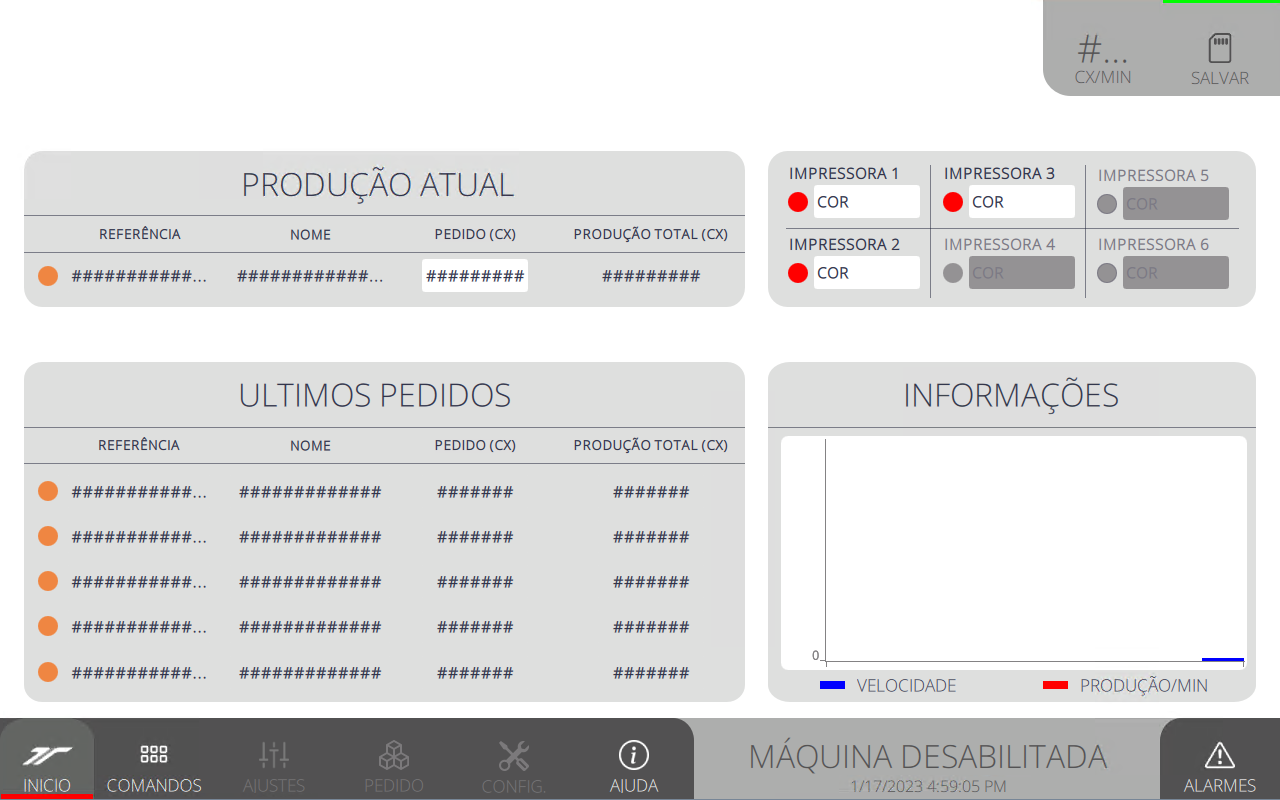
\includegraphics[width=480px,height=300px]{src/imagesFlexo/01-main/e-Tela-Principal.png}
  \caption{Tela Principal.}
   \label{}
\end{figure}

\newpage
\thispagestyle{fancy}

\vspace*{\fill}

\subsubsection{\small{Gráficos de velocidade e produção}}


\begin{figure}[h]
  \centering
  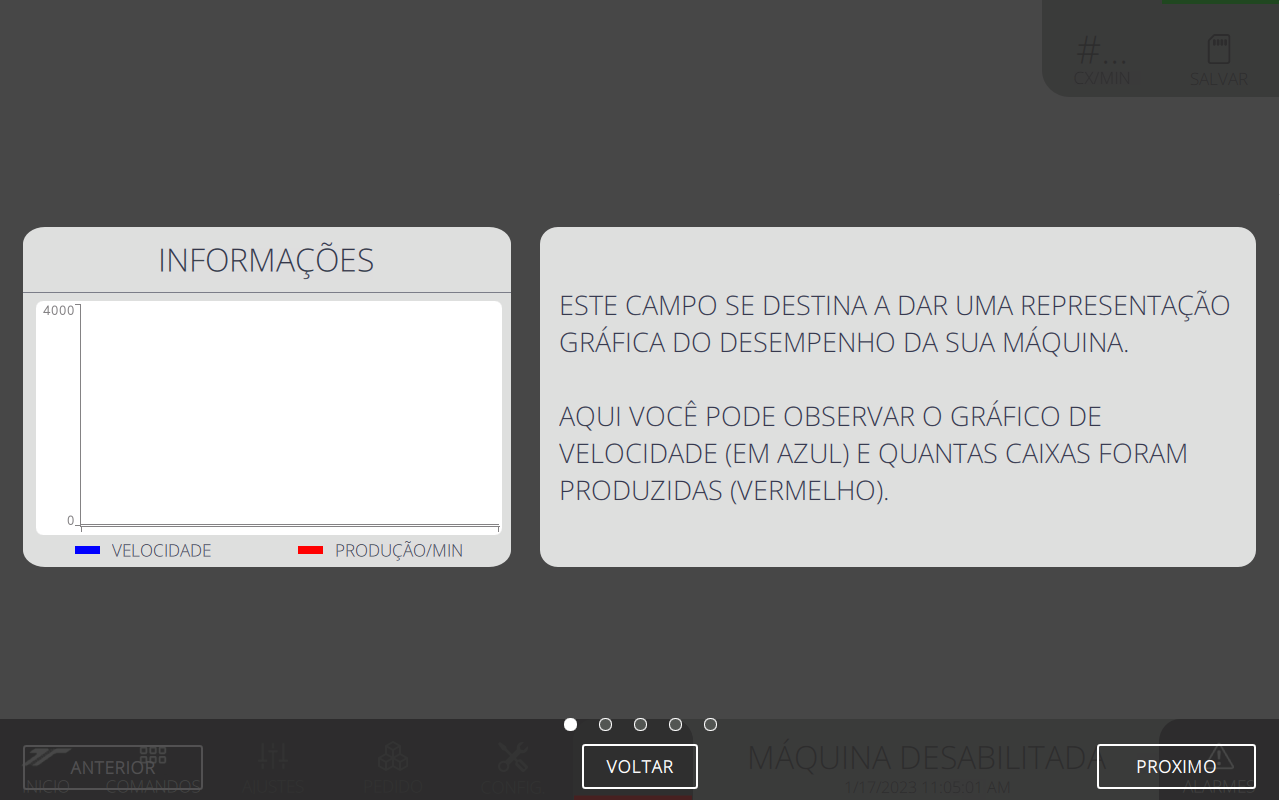
\includegraphics[width=576px,height=360px]{src/imagesFlexo/01-main/e-1.png}
  \caption{ver depois.}
   \label{}
\end{figure}

\vspace*{\fill}

\newpage
\thispagestyle{fancy}

\vspace*{\fill}

\subsubsection{\small{Informações sobre as impressoras}}


\begin{figure}[h]
  \centering
  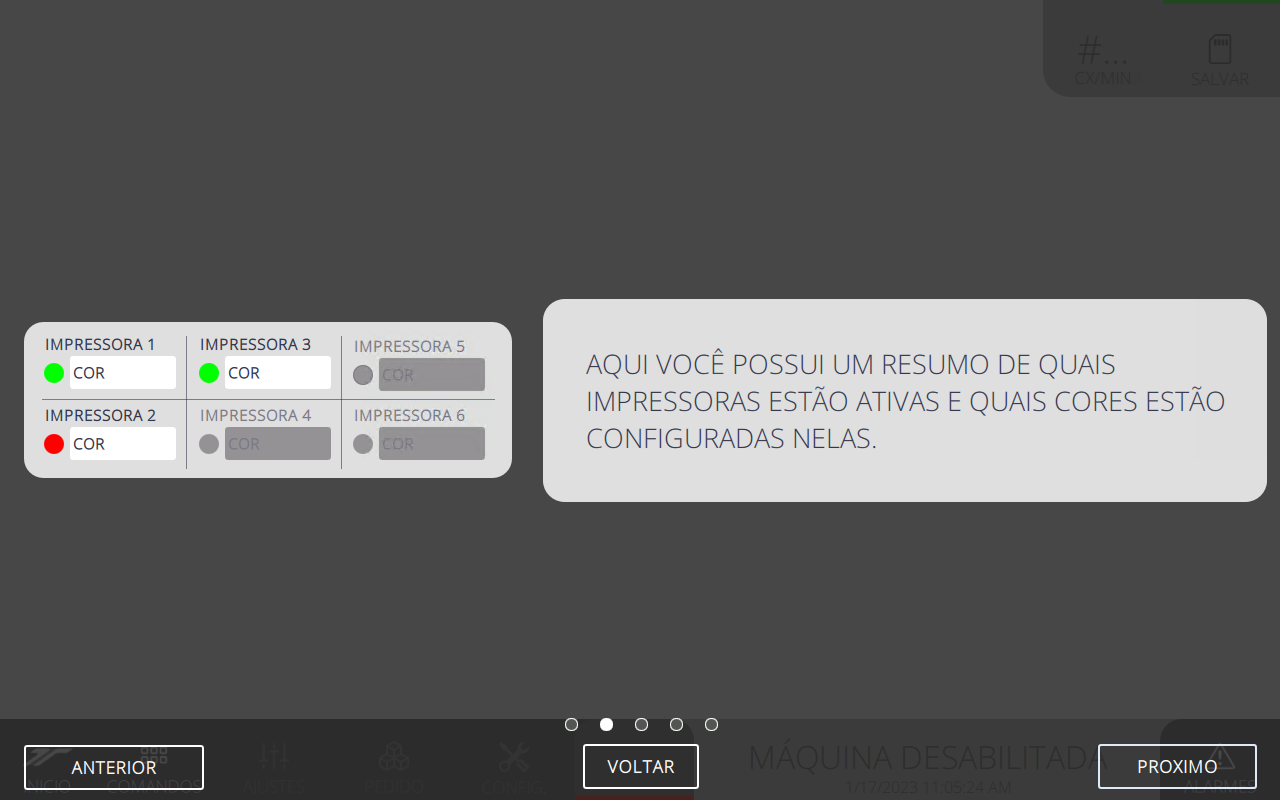
\includegraphics[width=576px,height=360px]{src/imagesFlexo/01-main/e-2.png}
  \caption{ver depois.}
   \label{}
\end{figure}

\vspace*{\fill}

\newpage
\thispagestyle{fancy}

\vspace*{\fill}

\subsubsection{\small{Ultimo pedido sem informação}}


\begin{figure}[h]
  \centering
  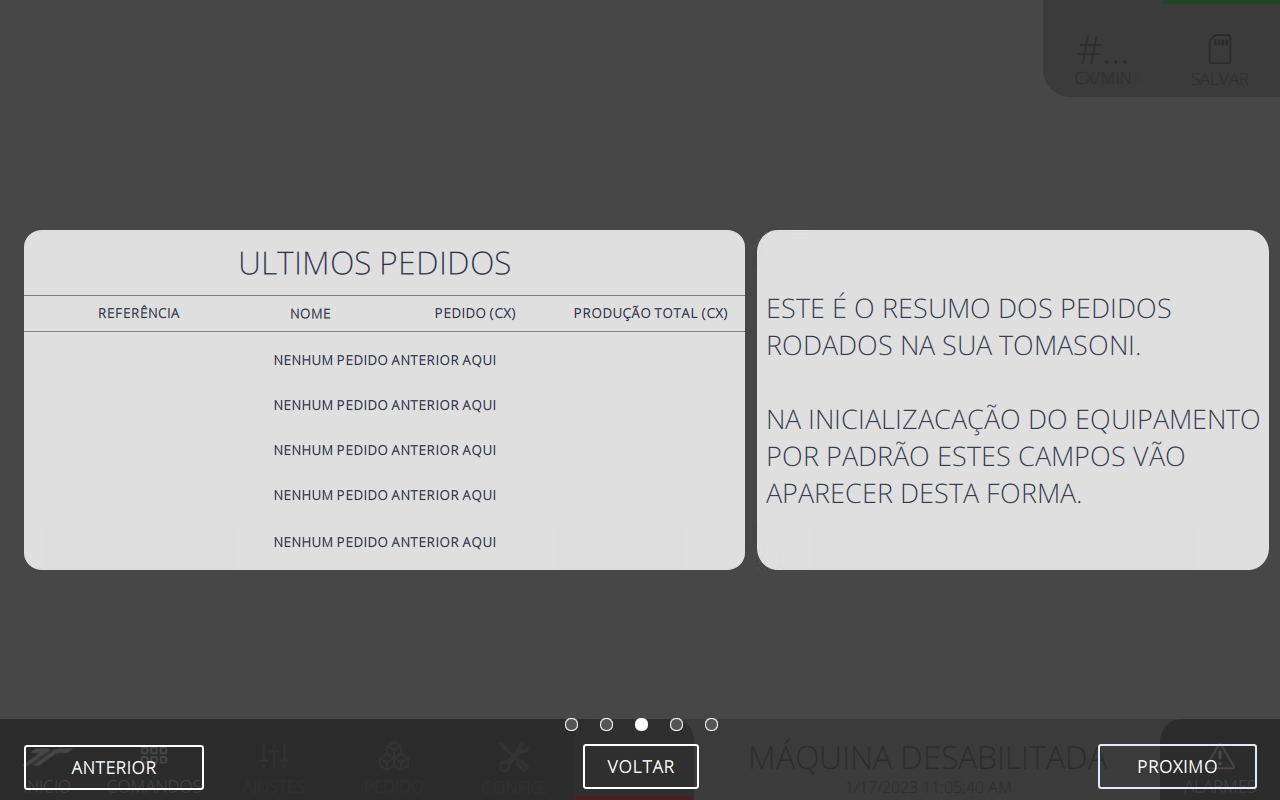
\includegraphics[width=576px,height=360px]{src/imagesFlexo/01-main/e-3.png}
  \caption{ver depois.}
   \label{}
\end{figure}

\vspace*{\fill}



\newpage
\thispagestyle{fancy}

\vspace*{\fill}

\subsubsection{\small{Ultimo pedido}}


\begin{figure}[h]
  \centering
  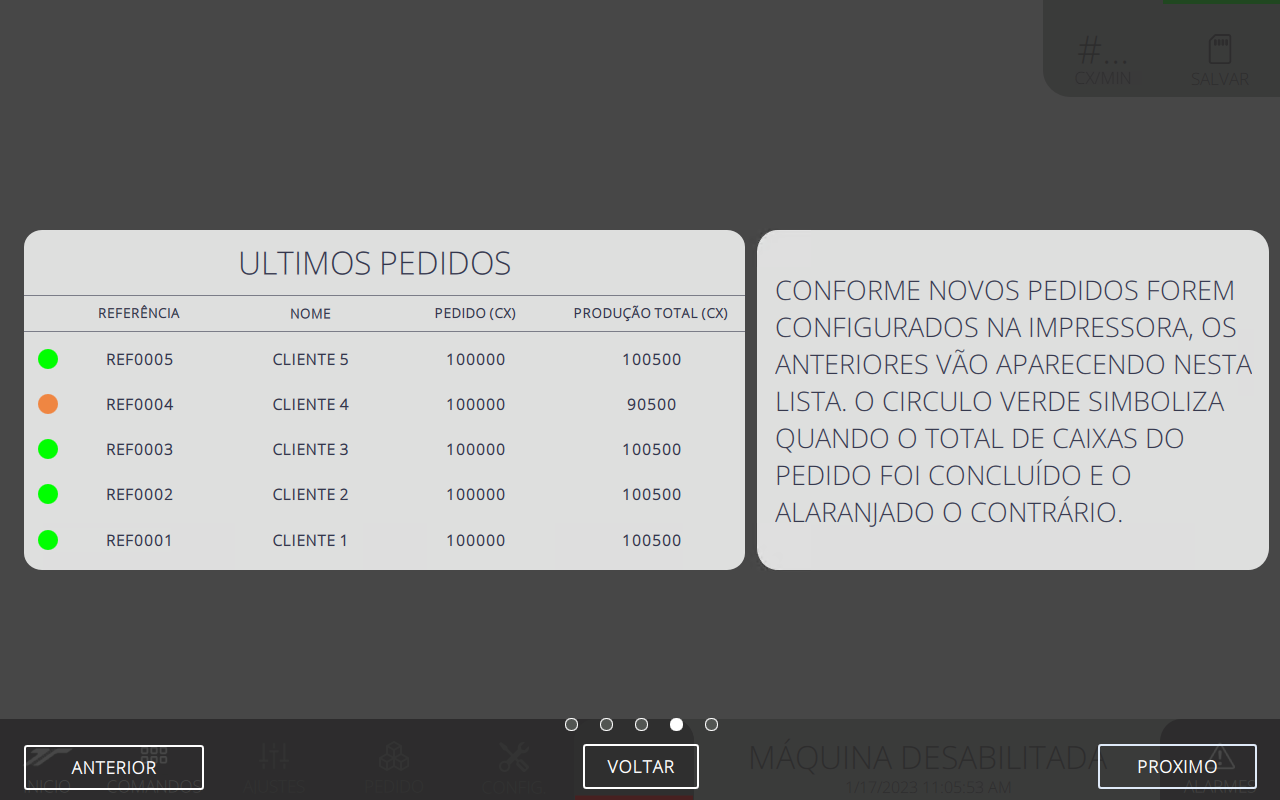
\includegraphics[width=576px,height=360px]{src/imagesFlexo/01-main/e-4.png}
  \caption{ver depois.}
   \label{}
\end{figure}

\vspace*{\fill}
\newpage
\thispagestyle{fancy}

\vspace*{\fill}

\subsubsection{\small{Pedido atual sem informação}}

\begin{figure}[h]
  \centering
  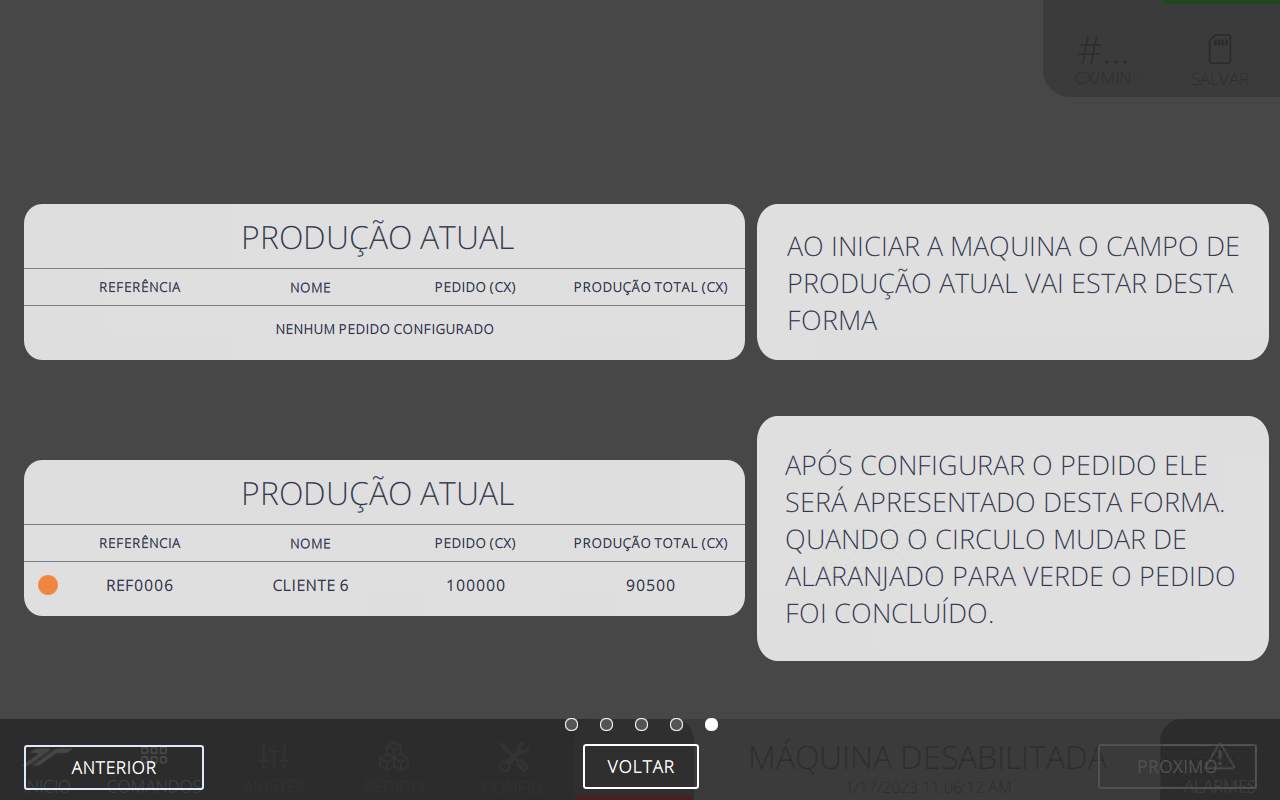
\includegraphics[width=576px,height=360px]{src/imagesFlexo/01-main/e-5.png}
  \caption{ver depois.}
   \label{}
\end{figure}

\vspace*{\fill}